\chapter{\selectlanguage{greek}Θεωρητικό υπόβαθρο}

Στο κεφάλαιο αυτό παρουσιάζονται αναλυτικά οι ...

\section{\selectlanguage{greek}\en{Deep Learning}}

Η υπολογιστική εκμάθηση \en{(Machine Learning)} είναι η κινητήριος δύναμη για διάφορες εκφάνσεις της σύγχρονης κοινωνίας: από αναζητήσεις στο διαδίκτυο μέχρι και φιλτράρισμα περιεχομένου σε κοινωνικά δίκτυα και προτάσεις αγορών σε ηλεκτρονικά καταστήματα. Ολοένα συχνότερη και συνηθέστερη γίνεται η εμφάνιση του σε προϊόντα ευρείας κατανάλωσης όπως κάμερες και κινητά τηλέφωνα. Τα συστήματα υπολογιστικής εκμάθησης χρησιμοποιούνται για την αναγνώριση αντικειμένων σε εικόνες, την αυτόματη καταγραφή προφορικού λόγου, την αντιστοίχηση προϊόντων, νέων, δημοσιεύσεων με τις προτιμήσεις χρηστών. Σε όλες αυτές τις εφαρμογές, είναι αυξανόμενη η χρήση ενός σετ τεχνικών που φέρει το όνομα \en{Deep Learning}.

Οι συμβατικές τεχνικές υπολογιστικής εκμάθησης είχαν περιορισμένη δυνατότητα χρήσης της ανεπεξέργαστης πληροφορίας. Για δεκαετίες, η σχεδίαση και η υλοποίηση ενός συστήματος αναγνώρισης προτύπων ή υπολογιστικής εκμάθησης, απαιτούσε προσεκτική προσέγγιση και σημαντική εξειδίκευση στον εκάστοτε τομέα. Αυτό επειδή χρειαζόταν η μετατροπή της ανεπεξέργαστης πληροφορίας σε μία κατάλληλη εσωτερική αναπαράσταση, την οποία το υποσύστημα εκμάθησης -- συχνότερα ένας ταξινομητής -- θα χρησιμοποιούσε για αναγνωρίσει πρότυπα στις διάφορες εισόδους.

Η εκμάθηση αναπαραστάσεων είναι ένα σύνολο μεθόδων που επιτρέπουν σε ένα σύστημα να ανακαλύψει αυτόματα ποιες ακριβώς αναπαραστάσεις της ανεπεξέργαστης πληροφορίας χρειάζεται για να επιτελέσει την αναγνώριση προτύπων ή την ταξινόμηση. Οι μέθοδοι \en{Deep Learning} είναι μέθοδοι εκμάθησης αναπαραστάσεων με πολλαπλά επίπεδα αναπαράστασης, που αποτελούνται από την σύνθεση απλών, μη γραμμικών υποσυστημάτων, το καθένα από τα οποία -- ξεκινώντας από την ανεπεξέργαστη είσοδο -- μετατρέπει την αναπαράσταση της πληροφορίας σε μια λίγο πιο υψηλά αφαιρετική μορφή σε κάθε επίπεδο. Με την χρήση αρκετών τέτοιων μετατροπών το σύστημα μπορεί να μάθει εξαιρετικά σύνθετες λειτουργίες. Για διαδικασίες ταξινόμησης, τα υψηλότερα επίπεδα αναπαράστασης ενισχύουν πτυχές τις εισόδου που είναι πιο σημαντικές για τον τελικό σκοπό. Σε μία εικόνα, για παράδειγμα, η οποία αναπαριστάται ως διάνυσμα τιμών εικονοκυττάρων, τα χαρακτηριστικά που μαθαίνονται στο πρώτο επίπεδο είναι συνήθως πληροφορία για την παρουσία ή την απουσία ακμών σε συγκεκριμένες θέσεις και προσανατολισμούς. Στο δεύτερο επίπεδο, συνήθως εντοπίζονται μοτίβα μέσω των διαφόρων διατάξεων των ακμών, χωρίς να χρειάζεται τα μοτίβα να επαναλαμβάνονται επακριβώς. Στο τρίτο επίπεδο μπορούν να αναγνωριστούν σύνολα μοτίβων σε μεγάλους συνδυασμούς που αντιστοιχούν σε γνωστά αντικείμενα ή μέρη τους. Τα επόμενα επίπεδα, παρόμοια, εντοπίζουν πιο σύνθετα αντικείμενα ως συνδυασμούς απλούστερων μερών. Το βασικότερο στοιχείο του \en{Deep Learning} είναι πως τα επίπεδα που εντοπίζουν χαρακτηριστικά και δομές δεν είναι σχεδιασμένα από τους ανθρώπους: μαθαίνονται από τα δεδομένα χρησιμοποιώντας γενικευμένες διαδικασίες εκμάθησης.

Η χρήση του \en{Deep Learning} έχει βοηθήσει στην αντιμετώπιση προβλημάτων που δυσκόλευαν την κοινότητα της τεχνητής νοημοσύνης εδώ και χρόνια. Αποδεικνύεται να έχει επιδόσεις χωρίς προηγούμενο στον εντοπισμό πολύπλοκων δομών σε δεδομένα πολλών διαστάσεων και για αυτό είναι εφαρμόσιμο σε πολλούς διαφορετικούς τομείς, επιστημονικούς, επιχειρησιακούς και κοινωνικοπολιτικούς. Πέρα από επαναστατικές επιδόσεις στην αναγνώριση φωνής και εικόνας, έχει ξεπεράσει άλλες τεχνικές υπολογιστικής εκμάθησης στην πρόβλεψη συμπεριφοράς μορίων φαρμάκων, στην ανάλυση δεδομένων από επιταχυντές σωματιδίων, στην ανακατασκευή εγκεφαλικών κυκλωμάτων και στην πρόβλεψη των επιπτώσεων μεταλλάξεων μη κωδικοποιητικού \en{DNA} στις γονιδιακές εκφράσεις και ασθένειες. Ίσως, οι πιο αναπάντεχα υποσχόμενες επιδόσεις έγιναν στον κλάδο της επεξεργασίας φυσικής γλώσσας, συγκεκριμένα στην εντοπισμό θεμάτων, την ανάλυση συναισθήματος, τις ερωτήσεις - απαντήσεις και την μετάφραση.
%TODO References for best results from paper Deep Learning Hinton Bengio lecun

\section{\selectlanguage{greek} \en{Supervised Learning}}

Η πιο συνήθης μορφή υπολογιστικής εκμάθησης, είτε \en{Deep Learning} είτε όχι, είναι αυτή της επιτηρούμενης εκμάθησης. Ας θεωρήσουμε πως θέλουμε να φτιάξουμε ένα σύστημα που αποφασίζει τι περιέχει μια εικόνα, όπως ένα σπίτι, ένα αυτοκίνητο, έναν άνθρωπο ή μία γάτα. Αρχικά, συλλέγουμε ένα αρκετά μεγάλο σύνολο δεδομένων με εικόνες στα οποία σημειώνεται τι αντικείμενο από τα παραπάνω περιέχει κάθε εικόνα. Κατά τη διάρκεια της εκπαίδευσης δείχνουμε στο σύστημα μια εικόνα και αυτό παράγει μία πρόβλεψη, στη μορφή ενός διανύσματος με σκορ για κάθε κατηγορία. Θέλουμε η επιθυμητή κατηγορία να έχει το μεγαλύτερο σκορ πρόβλεψης αλλά αυτό είναι πολύ δύσκολο πριν την εκπαίδευση. Υπολογίζουμε μία αντικειμενική %TODO What is an objective function
Ο \en{CLIC -- Compact Linear Collider} -- αποτελεί μια μελέτη για ένα μελλοντικό επιταχυντή που θα φτάσει σε πρωτοφανή επίπεδα ενέργειας ηλεκτρόνια και αντισωμάτιά τους, ποζιτρόνια. 
Όταν θα έρχονται σε επαφή μέσω σύγκρουσης, θα καταστρέφουν το ένα το άλλο, απελευθερώνοντας όλη τους την ενέργεια για την παραγωγή νέων σωματιδίων.

Τα ηλεκτρόνια και τα ποζιτρόνια είναι θεμελιώδη σωματίδια και οι συγκρούσεις τους μπορούν να προσφέρουν εξαιρετικά λεπτομερείς πληροφορίες σχετικά με τους νόμους της φύσης. 
Έτσι ο \en{CLIC} θα προσφέρει σημαντικές θεμελιώδεις γνώσεις φυσικής, πέρα από αυτές που είναι διαθέσιμες από το Μεγάλο Επιταχυντή Αδρονίων (\en{Large Hadron Collider -- LHC}) ή από ένα γραμμικό επιταχυντή ηλεκτρονίων/ποζιτρονίων χαμηλότερης ενέργειας, λόγω του μοναδικού συνδυασμού πειραματικής ακρίβειας και υψηλής ενέργειας.

Σε αυτές τις υψηλές ενέργειες, τα ηλεκτρόνια και ποζιτρόνια θα έχαναν ένα τεράστιο μέρος της ενέργειάς τους επιταχυνόμενα σε έναν κυκλικό επιταχυντή σαν τον \en{LHC}. 
Έτσι, τα σωματίδια πρέπει να επιταχυνθούν σε δύο γραμμικούς επιταχυντές που αντικρίζουν ο ένας τον άλλο, έτσι ώστε οι δέσμες να συγκρούονται στον κεντρικό ανιχνευτή. 
Αυτό συνεπάγεται ότι τα σωματίδια πρέπει να αποκτήσουν την ενέργειά τους από ένα και μόνο πέρασμα τους μέσα από τις κοιλότητες επιτάχυνσης.

\begin{figure}[h]
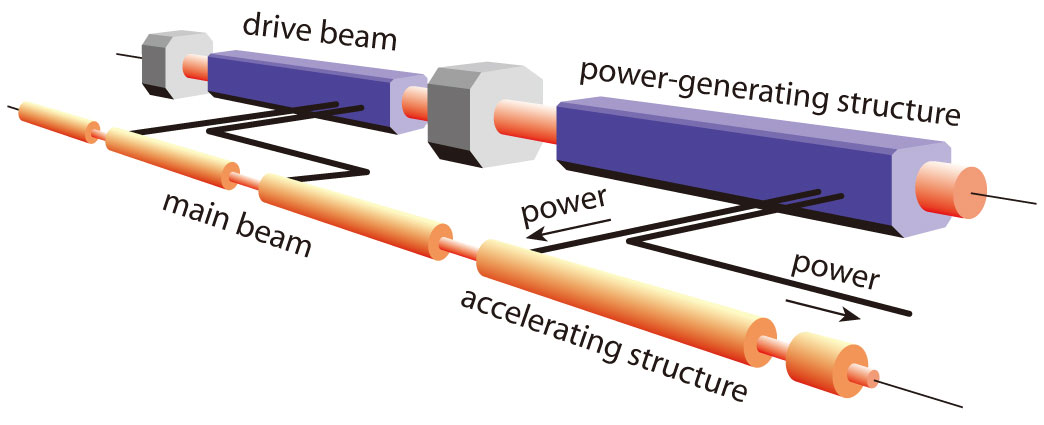
\includegraphics[width=0.5\textwidth]{images/CLIC-twobeam.jpg}
\centering
\caption{Το σύστημα δύο δεσμών του \en{CLIC}}
\label{CLICtwobeamscheme}
\end{figure}

Ο \en{CLIC} έχει σχεδιαστεί για να κατασκευαστεί σε στάδια αυξανόμενης ενέργειας για σύγκρουση: ξεκινώντας από \SI{360}{\GeV}, περίπου \SI{1.4}{\TeV}, και μέχρι την τελική ενέργεια των \SI{3}{\TeV}. 
Προκειμένου να επιτευχθεί αυτή η ενέργεια με ένα ρεαλιστικό και οικονομικά αποδοτικό τρόπο, η αύξηση της επιτάχυνσης πρέπει να είναι πολύ υψηλή.
Ο \en{CLIC} αποσκοπεί σε επιτάχυνση των \SI[per-mode = symbol]{100}{\mega \volt \per \metre}, 20 φορές υψηλότερη από αυτή του \en{LHC}.

Αυτή η δέσμη-οδηγός (drive beam) επιβραδύνεται σε ειδικές Διατάξεις Εξαγωγής και Mεταφοράς Ισχύος -- \en{Power Extraction and Transfer Structures (PETS)}, και η παραγόμενη \en{RF} ισχύς μεταφέρεται στην κύρια δέσμη. 
Αυτό οδηγεί σε μια πολύ απλή διάταξη σήραγγα χωρίς ενεργά \en{RF} μέρη (δηλ. \en{klystrons}).

\begin{figure}[h]
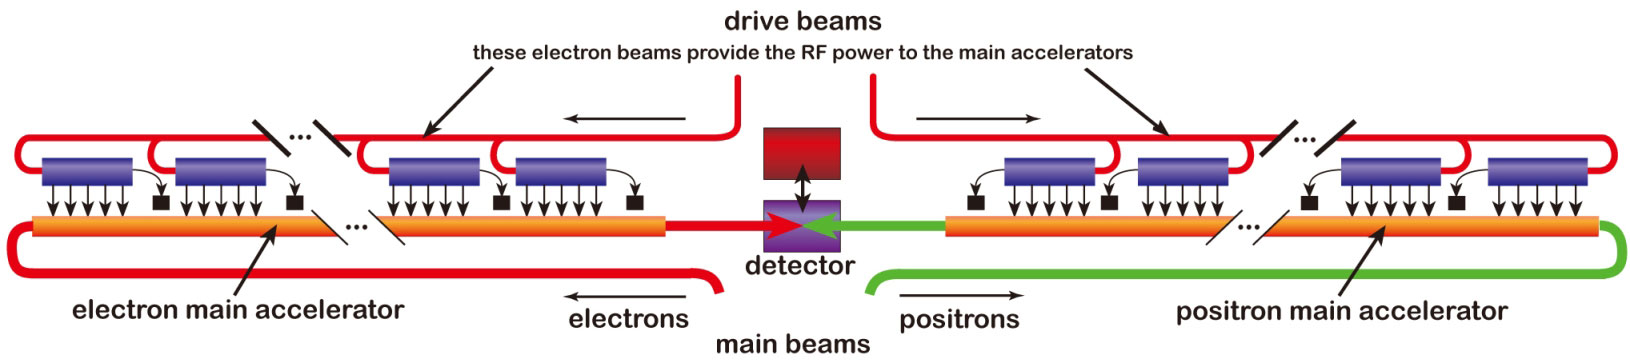
\includegraphics[width=\textwidth]{images/CLIC-layout.jpg}
\centering
\caption{Το σχεδιάγραμμα του \en{CLIC}}
\label{CLIClayout}
\end{figure}

Ο \en{CLIC} είναι μία από τις επιλογές για έναν μελλοντική επιταχυντή κατασκευασμένο στο \en{CERN}, το οποίο θα αποφασιστεί ανάλογα με τα μελλοντικά αποτελέσματα του \en{LHC}.

\section{\selectlanguage{greek}Το \en{Electron beam scanner}}

